\subsection*{Обработка данных}


\textbf{Погрешнсть измерений}. Для начала заметим, что процесс рассеяния носит вероятностный характер, так что, возможно, адеквантно оценивать погрешность измерения $N$, как $\sqrt{N}$. Проверим это, рассмотрев $\sigma$  для свинца, и сравнив с $\sqrt{N}$ для соответствующего результата. Значения $\sigma / \sqrt{N}$ лежат в диапазоне $[0.2,\, 0.6]$, что говорит об адекватности оценки погрешности, как по $\sqrt{N}$.

При измерениях в некоторый промежуток времени получалось бы, что 
\begin{equation}
    N_1 = \frac{N}{t}, \hspace{5 mm} 
    \sigma_{N_1} = \frac{1}{t}\left(N \pm \sqrt{N}\right),
    \hspace{0.5cm} \Rightarrow \hspace{0.5cm}
    \sigma^{\text{True}}_{N_1} = \frac{\sqrt{N}}{t},
    \label{err}
\end{equation}
но так как $t \sim 10$ для большинства измерений, оставим оценку погрешности, как $\sqrt{N/t}$.



Измерения длины препятствий будут складываться. Считая, что погрешность измерения каждого кусочки $\sigma_{l_1} = 0.2$ мм, может найти, что $\sigma_{n * l} = n \sigma_{l_1}$,
где $n$ -- количество кусочков. 



\textbf{Коэффициент ослабления}. Из формулы \eqref{base}, можем найти, что
\begin{equation*}
    \ln \frac{N_0}{N} = \mu l,
\end{equation*}
так что построим данные из таблицы \ref{tab:1} в логарифмическом масштабе (рис. \ref{fig:1}).

\vspace{-1cm}

\begin{figure}[h]
    \centering
    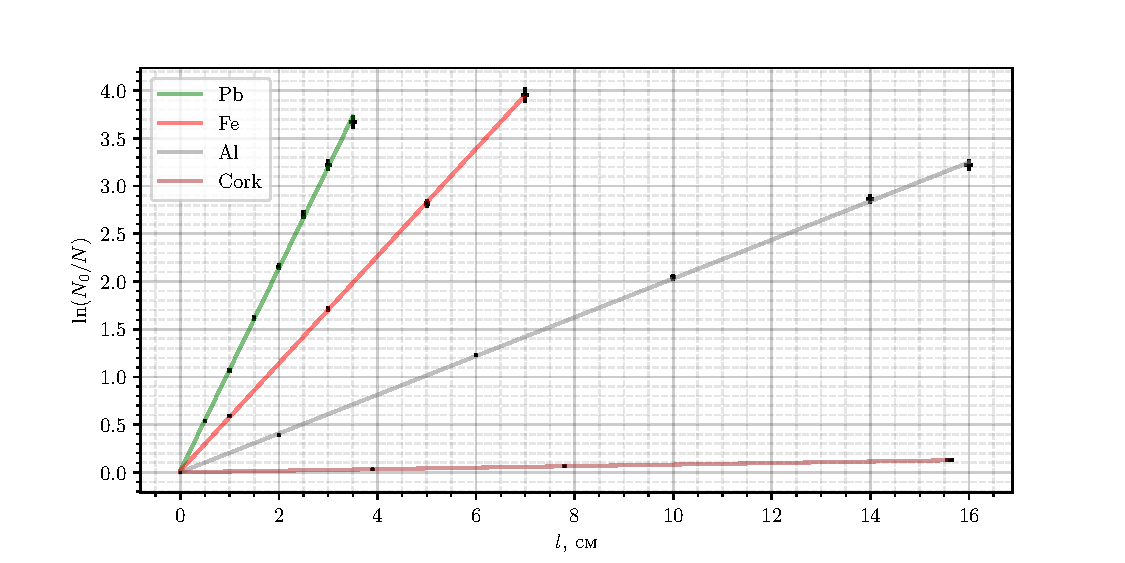
\includegraphics[width=0.95\textwidth]{figures/plot511.pdf}
    \caption{Зависимость детектированных в секунду $\gamma$-частиц, от толщины образца}
    \label{fig:1}
\end{figure}


Из полученной завимисти можем оценить $\chi^2/\text{ndf}$, а также найти через линейную регрессию значения $\mu$ для различных материалов. Результаты приведены в таблице \ref{tab:2}.





\begin{table}[h!]
    \centering
    \caption{Измеренные значения $\mu$ и оценки $\chi^2/\text{ndf}$}
\begin{tabular}{lrrr}
\toprule
    &  $\mu$, м$^{-1}$ &  $\sigma$, м$^{-1}$ &  $\chi^2$ \\
\midrule
  Pb &  101.2 &       0.9 &      0.68 \\
  Fe &   56.3 &       0.3 &      1.10 \\
  Al &   20.3 &       0.1 &      0.55 \\
Cork &    0.80 &       0.02 &      0.03 \\
\bottomrule
\end{tabular}
\label{tab:2}
\end{table}


По рисунку \ref{fig:3} можно восстановить, что для алюминия и железа такие значения коэффициентов ослабления соответсвуют энергии в 
\begin{equation*}
    E \approx 0.8 \text{ МэВ},
\end{equation*}
однако для свинца получился коэффицент ослабления $E \approx 0.7$ МэВ, что в контексте большой производной этого участка графика вполне позволяет сказать,  о том что в пределах погрешности указанное значение $E$ совпало для всех трёх веществ.

